\documentclass[11pt, intlimits]{beamer}
\usepackage[utf8]{inputenc}
\usepackage[T1, T2A]{fontenc}
\usepackage[english, russian]{babel}
\usepackage{moreverb}
\usepackage{array}
\usepackage{hyperref}
\usepackage{amsthm}
\usepackage{wrapfig}
\pdfmapfile{+sansmathaccent.map}
\mode<presentation>{
 \usetheme{Frankfurt}
 \setbeamertemplate{navigation symbols}{}
 \setbeamertemplate{footline}[frame number]
}
%\expandafter\def\expandafter\insertshorttitle\expandafter{%
%   \insertshorttitle\hfill%
%   \insertframenumber\,/\,\inserttotalframenumber}
\setcounter{tocdepth}{2}
\graphicspath{{fig/}}
\newcommand{\Expect}{\mathsf{E}}
\DeclareGraphicsExtensions{.png,.jpg}
\DeclareMathOperator*{\toplim}{\overline\lim}
\DeclareMathOperator*{\botlim}{\underline\lim}
\DeclareMathOperator*{\tou}{\longrightarrow}
% Титульный лист
\title{Нейронные сети для изображений}
\institute{%
    Санкт-Петербургский государственный университет \\
    Математико-механический факультет \\
    Статистическое моделирование
}
\author{Старков Артём, гр. 622}
\date{
    Санкт-Петербург\\
    \number\year
}
\begin{document}

% 1 Заголовочный
\begin{frame}
    \titlepage
\end{frame}

\section{Задача}
% 2 Задача
\begin{frame}{Постановка задачи классификации в нейросетях}

Классификация на $M$ классов. Пусть $\mathcal{X}$ -- множество значений индивидов $x$, $\mathcal{Y}$ -- множество классов $y$. Имеем неизвестную зависимость
$$
y=f(x), f: \mathcal{X} \to \mathcal{Y}.
$$

Зафиксируем $X \subset \mathcal{X}$, для которых $f(x)$ известно. Получаем задачу классификации с учителем; ищем $f^*(x)$, чтобы функционал качества 
$$
Q(f^*, X)=\frac{1}{m}\sum_{x\in X} \mathcal{L}(f^*(x), f(x))
$$
достигал минимума на $X$.
\end{frame}


% 3 Задача (2)
\begin{frame}{Постановка задачи классификации в нейросетях}

Метод минимизации эмпирического риска:
$$
f^*=\arg\min_{f'\in \mathcal{F}} Q(f', X),
$$
где $\mathcal{F}$ -- класс функций, аппроксимирующих целевую функцию $f(x)$.

Для нейронных сетей задача решается для параметризованных аппроксиматоров $f^*(x; \theta)$ путем подбора параметров весов:
$$
\min_{\theta} \frac{1}{m}\sum_{x\in X} \mathcal{L}(f^*(x; \theta), f(x)).
$$
Многослойные сети: на вход следующих слоев подается выход из предыдущих через нелинейность $\sigma(.)$.
\end{frame}

% 4 Особенности
\begin{frame}{Особенности при применении к изображениям}
При применении данной задачи к изображениям обнаруживается ряд особенностей, позволяющих обособить эту задачу от других:

\begin{itemize}

\item локальная скоррелированость пикселей;
\item распределенность признака: один пиксель практически не несет в себе информации, признак на изображении -- это совокупность пикселей;
\item возможные трансформации детектируемых шаблонов: поворот, масштабирование, смещение, перекрытие другими предметами сцены и др.

\end{itemize}
\end{frame}

\section{Основные элементы}

% 5 Свертка
\begin{frame}{Свертка}
Свертка помогает выделить признаки из совокупности пикселей. Свертка функций $f$ и $w$ по области $D$:
$$
(f*w)(x)=\int_D f(y)w(x-y)dy=\int_D f(x-y)w(y)dy;
$$

Например, пусть $f:Z \times Z \to R^K, w: D \times D \to R^K, D = 1..d$ (свертка изображения по ядру $w$ размером $d \times d$ и глубины каналов $K$):
$$
(f*w)(i,j)=\frac{1}{Kd^2}\sum_{k=1}^K \sum_{t,n =1}^d f_k(i-t, j-n) w_k(t,n).
$$


\end{frame}

% 6 Feature map
\begin{frame}{Feature map (activation map)}

Пусть на вход подается изображение размером $M \times N$. Обозначим его как отображение $x: Z \times Z \to R^3$.
Введем ядро свертки, представляющее собой набор весов $W: Z \times Z \to R^3$. Рассмотрим следующее отображение:
$$
f(i, j): Z \times Z \to R;
$$
$$
f(i, j) = \sigma((W*x)(i, j) + b);
$$
где $b$ --- некоторое смещение, $\sigma$ --- нелинейная функция. Вектор из таких отображений, построенный на \textit{разных} ядрах $W_k$ и смещениях $b_k$ называется \textbf{feature map}. 

\end{frame}

% 6.1 сверточный слой
\begin{frame}{Сверточный слой}

Сверточный слой: 
\begin{itemize}
\item входная feature map 
$$
f^{(s-1)}(i, j) \in R^{N^{(s-1)} \times N^{(s-1)} \times K^{(s-1)}};
$$

\item $K^{(s)}$ обучаемых ядер 
$$
W \in R^{d \times d \times K^{(s-1)}};
$$

\item $K^{(s)}$ смещений 
$$
b^{(s)} \in R;
$$

\item выходная feature map, подаваемая на вход следующего слоя: 
$$
f^{(s)}(i, j) \in R^{N^{(s)} \times N^{(s)} \times K^{(s)}};
$$

\end{itemize}

Внешние параметры слоя: глубина feature map $K^{(s)}$, размер ядра $d^{(s)}$, нелинейность $\sigma(.)$.

\end{frame}


% 7 ReLU
\begin{frame}{Rectifier linear unit (ReLU)}

В сверточных сетях функцией активации чаще всего выбирают Rectifier linear unit (ReLU): $$f(x)=\max(x, 0).$$

Softplus -- гладкий ReLU:
$$
f(x)=\ln(1+e^x).
$$

\textbf{Плюсы:} очень просто вычисляемая производная: $(max(0, x))'=\gamma(x>0)$; нет проблемы vanishing gradient справа.

\textbf{Минусы:} проблема <<мертвых нейронов>>: нейрон может достичь состояния, когда градиент становится нулевым, и обучения больше не происходит.

\end{frame}

% 8 ReLU вариации
\begin{frame}{Варианты ReLU}

Варианты ReLU для избежания проблемы <<мертвых нейронов>>:
\begin{itemize}

\item Leaky ReLU ($\epsilon > 0$ -- входной параметр): 
$$
f(x)=
\begin{cases}
x, & x \ge 0, \\
\epsilon x & x < 0.
\end{cases}
$$

\item Shifted ReLU ($\alpha > 0$ -- входной параметр): 
$$
f(x)=\max(x, 0) - \alpha.
$$

\item Exponential ReLU (ELU) ($a > 0$ -- обучаемый параметр):
$$
f(x)=
\begin{cases}
x, & x \ge 0, \\
a(e^x-1) & x < 0.
\end{cases}
$$

\end{itemize}

\end{frame}

% 9 Пулинг
\begin{frame}{Субдискретизация (pooling)}

\textbf{Слой пулинга (pooling)}: нелинейное уплотнение карты признаков. для снижения размерности и выявления новых признаков на больших расстояниях.
$$
maxpool(x)(i, j)=\max\left(\left\{x(i+t,j+n)\right\}_{t,n=1}^{d}\right),
$$
где $d \times d$ -- размер ядра пулинга. 

\begin{figure}[h]
\center{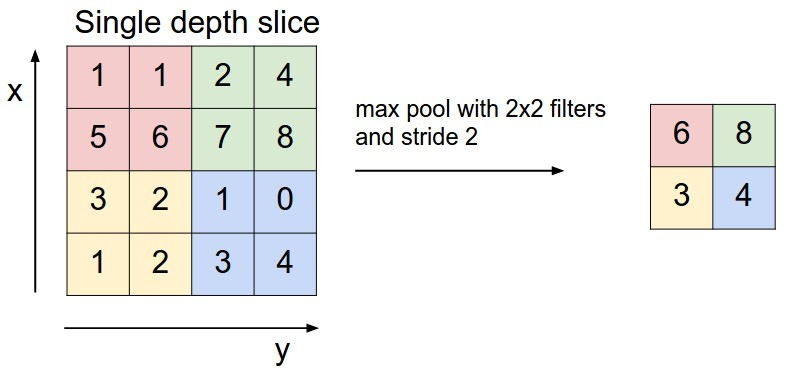
\includegraphics[width=0.7\linewidth]{maxpool}}
\caption{Max pooling на одном слое с ядром $2 \times 2$}
\label{img:lenet}
\end{figure}
\end{frame}

\section{LeNet, AlexNet}

% 10 DropOut, Data augmentation
\begin{frame}{Data augmentation, DropOut}

\begin{definition}{Data augmentation}
(увеличение данных) --- техника расширения пространства обучающих индивидов (изображений) путем применения аффинных преобразований и некоторых специфических приемов, например генерация изображений. Например, поворот изображения на некоторый угол, изменение размера изображения и др.
\end{definition}

% https://www.cs.toronto.edu/~hinton/absps/JMLRdropout.pdf
\begin{definition}{DropOut}
--- техника для регуляризации обычной сети: вводится новая модель нейрона, где каждый нейрон имеет вероятность $p$ не участвовать в следующей эпохе обучения сети; $p$ --- общий внешний параметр. В рабочем режиме $p=1$. В некотором смысле данная техника эквивалентна обучению множества нейросетей и усреднению результата. 
\end{definition}


\end{frame}

% 11 LeNet
\begin{frame}{Архитектура LeNet}

Архитектура LeNet: Yann LeCun et al.(1998). Параметры:
\begin{itemize}
\item 2 сверточных слоя, 2 max-pooling, 3 полносвязных, 10 классов на выходе;
\item 60 тыс. весов, из них 3 тыс. для сверточных слоев, остальные для полносвязных.
\end{itemize}

\begin{figure}[h]
\center{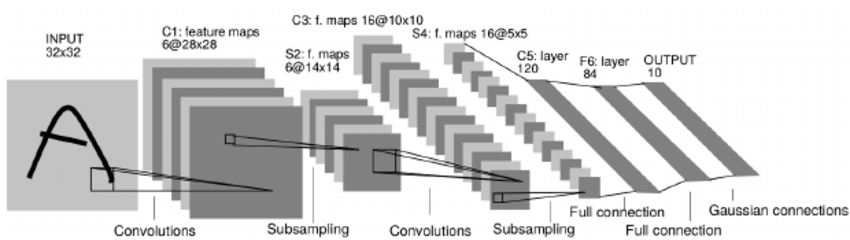
\includegraphics[width=1\linewidth]{lenet}}
\caption{Архитектура LeNet}
\label{img:lenet}
\end{figure}

\end{frame}

% 12 AlexNet
\begin{frame}{Архитектура AlexNet}

Архитектура AlexNet: Alex Krizhevsky et al.(2012). Параметры:
\begin{itemize}
\item 60 млн. весов, из них 4 млн. для сверточных слоев;
\item 5 сверточных слоев, 3 max-pooling, 3 полносвязных, 1000 классов на выходе;
\item ReLU, DropOut ($p=0.5$), data augmentation.
\end{itemize}

\begin{figure}[h]
\center{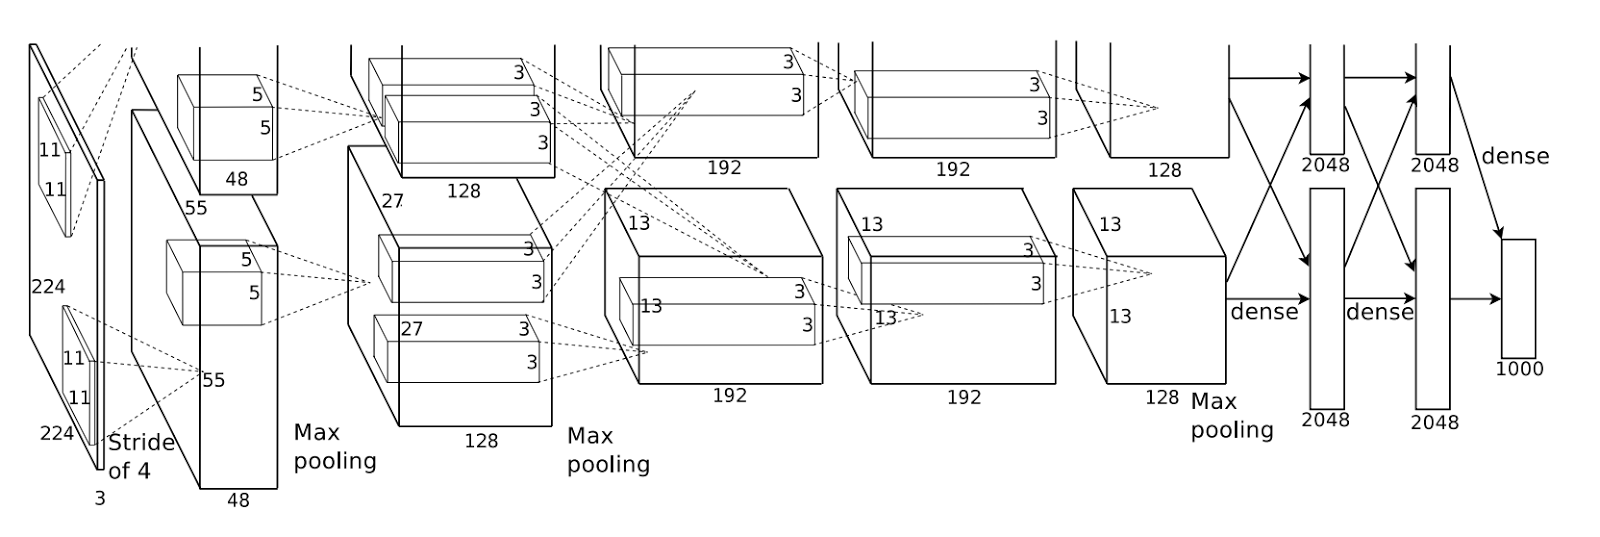
\includegraphics[width=1\linewidth]{alexnet}}
\caption{Архитектура AlexNet}
\label{img:alexnet}
\end{figure}


\end{frame}

\section{Inception}

% 13 Свертка 1х1
\begin{frame}{Свертка $1 \times 1$}

Пусть $f(i,j) : Z \times Z \to R^K$ -- сверточный слой; $x(i, j)$ -- вход:
$$
f(i,j)=\sigma((W*x)(i,j) + b).
$$
Задача: заменить линейный классификатор более универсальным:
например, $n$-слойным перцептроном:
\begin{gather*}
f^{(1)}(i,j)=\sigma(W^{(1)} x(i,j) + b^{(1)}), \\
... \\
f^{(n)}(i,j)=\sigma(W^{(n)} f^{(n-1)}(i,j) + b^{(n)}).
\end{gather*}

При $n=1$ получаем сверточный слой $1 \times 1 \times K$ ценой возврата к линейной модели. Возможности:
\begin{itemize}
\item произвольное изменение глубины feature map;
\item агрегация коррелированных признаков и избавление от слабых признаков.
\end{itemize}

\end{frame}

% 14 Inception
\begin{frame}{Inception}
Проблема: определение оптимального размера ядра. Решение: использование разных сверток и пулинга и конкатенация выходов в общую feature map. Свертки $1 \times 1$ уменьшают размерность для ускорения вычислений.

\begin{figure}[h]
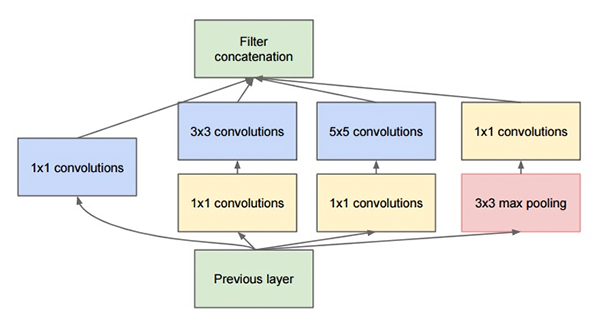
\includegraphics[width=0.7\textwidth]{inception_layer}
\caption{Архитектура блока Inception}
\label{img:inception_layer}
\end{figure}

\end{frame}


% 14.1 Inception
\begin{frame}{Архитектура GoogLeNet}
Архитектура GoogLeNet (2014). Параметры: 9 блоков Inception, 2 вспомогательных классификатора. Вход: $224 \times 224$, выход: 1000 классов.

\begin{figure}[h]
\center{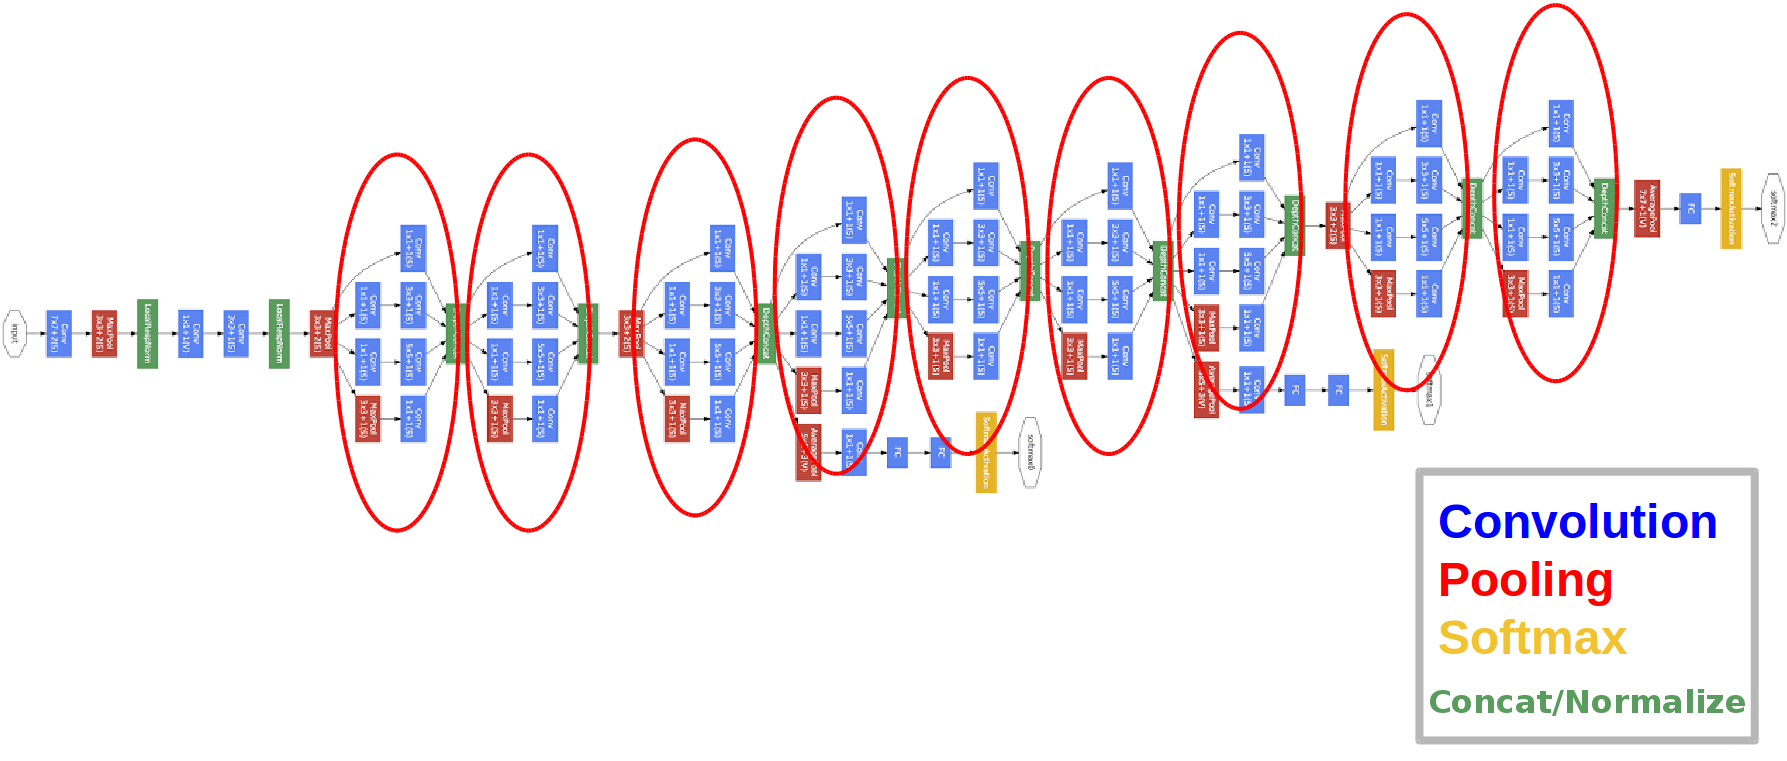
\includegraphics[width=1\linewidth]{googlenet}}
\caption{Архитектура GoogLeNet}
\label{img:googlenet}
\end{figure}

\end{frame}



\section{Batch normalization}

% 15 Внутренний ковариационный сдвиг
\begin{frame}{Внутренний ковариационный сдвиг}

Общая задача классификации с учителем:
$$
q(x|y)=p(y|x; \theta).
$$
На некоторой выборке $(X, Y)$ оптимизируем $\hat{\theta}$:
$$
\hat{\theta}=\arg \min Q(Y, \Expect[Y|X; \theta]).
$$

Для многослойной сети $x=\sigma(f^{(s-1)}), y=f^{(s)}, \hat{\theta}=W^{(s)}$. С увеличением количества шагов градиента распределение первого слоя стабилизируется, т.к. $\hat{\theta} \to \theta$. Однако вход второго слоя остается нестабилен до тех пор, пока 
$$
|\theta - \hat{\theta}|>\epsilon
$$
для некоторого $\epsilon > 0$. Эта проблема носит название внутреннего ковариационного сдвига. Способ решения: стандартизация входов.

\end{frame}

% 16 Batch normalization
\begin{frame}{Batch normalization}

Пусть:
\begin{itemize}
\item $f(i,j) : Z \times Z \to R^K$ --- feature map на входе слоя глубины $K$ и размерности $N \times M$;
\item $x=x_{i,j} \in R^{K}$ -- входные индивиды (пиксели).
\end{itemize}

Предполагаем:
$$
x \sim P(x; \Sigma, \mu) \ \ \ (K-\text{мерная.})
$$

Пусть $X \in R^{K \times MN}$ -- набор всех индивидов на $f(i, j)$. Тогда $\hat{\Sigma}$ --- оценка матрицы ковариации входа, $\hat{\mu}$ --- оценка смещения входа. Пересчет градиента такой модели требует вычисления:
$$
\frac{\partial}{\partial x} \hat{\Sigma}^{-1/2}(x-\hat{\mu}).
$$

\end{frame}

% 17 Batch normalization (2)
\begin{frame}{Batch normalization}

Предположим, что компоненты независимы, т.е. для $P(x; \Sigma, \mu) \ \Sigma$ диагональная:
$$
\Sigma=diag(\sigma_k^2).
$$
Стандартизуем покомпонентно:
$$
\bar{x}_{k, i} = \frac{x_{k, i} - \hat{\mu}_k}{\hat{\sigma}_k}.
$$
Проблема: ограниченность области значений $\bar{x}$. Решение: ввод линейной комбинации с обучаемыми параметрами:
$$
y_{k,i}=\gamma_k \bar{x}_{k,i} + \beta_k.
$$
Процедура BN сводится к удалению случайных параметров распределения входных данных и замене их на обучаемые.

\end{frame}

% 18 Batch normalization (3)
\begin{frame}{Batch normalization}

Отказ от смещения $b$ в модели нейрона ничего не изменит, но уменьшит количество параметров.

Возможности инструмента:
\begin{itemize}
\item регуляризация за счет исправления смещения;
\item общее ускорение обучения.
\end{itemize}

\begin{figure}[h]
\center{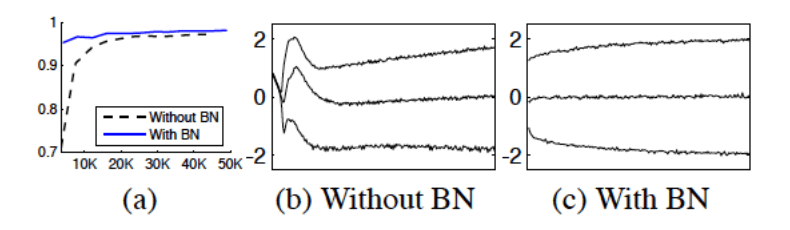
\includegraphics[width=1\linewidth]{bn}}
\caption{(a): изменение скорости обучения при использовании bn; 
(b, c): 15, 50 и 85-квантили для выходов одного из слоев в зависимости от эпохи}
\label{img:bn}
\end{figure}

\end{frame}

\section{ResNet}
% 20 ResNet, Inception ResNet 
\begin{frame}{Деградация сети}

Деградация сети: при увеличении количества слоев нейросети интуитивно логично ожидать улучшения качества предсказания, что в общем случае не так. Предполагаемые причины: затухание градиента.

\begin{figure}[h]
\center{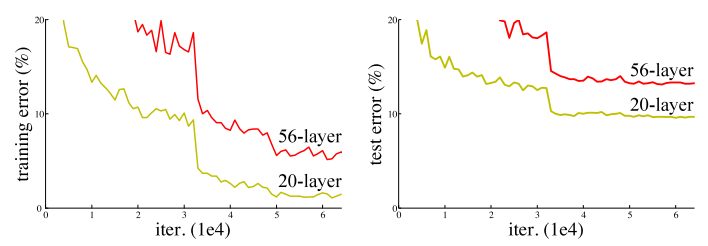
\includegraphics[width=1\linewidth]{degrade}}
\caption{Ошибка на тренировочной (a) и тестовой (b) выборках сети с 20 и 56 слоев}
\label{img:degrade}
\end{figure}

\end{frame}

% 20 ResNet, Inception ResNet 
\begin{frame}{Идея ResNet}

Решение как в бустинге: обучаться на остатках. Пусть аппроксимируем $\mathcal{H}(x)$ сетью $\mathcal{F}(x)$; предлагается использовать модель вида $\mathcal{H}(x)=\mathcal{F}(x)-x$.

\begin{figure}[h]
\center{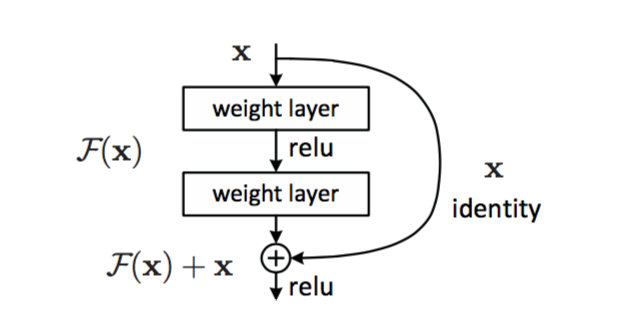
\includegraphics[width=0.4\linewidth]{resnet}}
\caption{Модель слоя с подключением ко входу}
\label{img:resnet}
\end{figure}

\end{frame}

% 20 ResNet, Inception ResNet 
\begin{frame}{Inception ResNet v2}

Архитектура сети Inception ResNet v2 (2016). Используются различные повторяющиеся блоки Inception с подключением выхода для вычисления остатков.

\begin{figure}[h]
\center{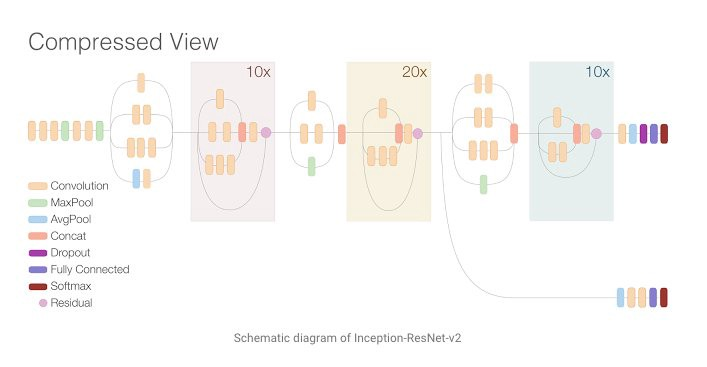
\includegraphics[width=0.8\linewidth]{IncResNet_v2}}
\caption{Архитектура сети Inception ResNet v2}
\label{img:IncResNet_v2}
\end{figure}

\end{frame}

% 20 DenseNet
\begin{frame}{DenseNet}

Изменен вид целевой функции алгоритма: на вход к текущему слою подаются выходы всех предыдущих:
$$
x^{(s)}=\mathcal{F}(x^{(1)}, x^{(2)}, ..., x^{(s-1)}),
$$

Глубина последнего слоя:
$
K^{(M)}=K^{(0)} + \sum_{s=1}^M K^{(s)},
$
где $K^{(0)}$ --- глубина входного слоя, $K^{(s)}$ --- глубина слоя $s$. Предлагается использовать неглубокие слои с малыми ядрами.

\begin{figure}[h]
\center{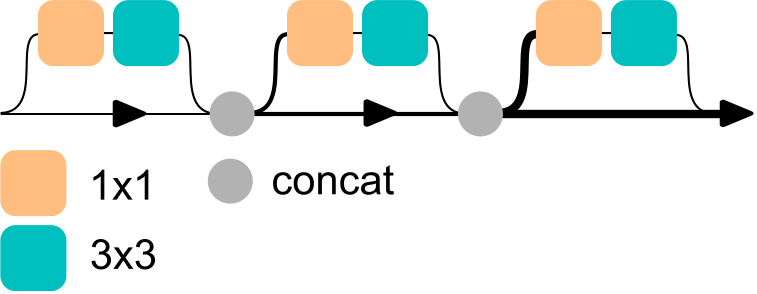
\includegraphics[width=0.6\linewidth]{densenet0}}
\caption{Схема блока DenseNet на трех слоях}
\label{img:densenet0}
\end{figure}

\end{frame}


\begin{frame}{DenseNet}

Архитектура сети DenseNet (2017). Используются различные повторяющиеся блоки Inception с подключением выхода для вычисления остатков.

Параметры: 4 <<Dense>> блока: на 6, 12, 24 и 16 слоев; переходные слои для уменьшения размерности. Вход $112 \times 112$, выход 1000 классов через полносвязный слой.

\begin{figure}[h]
\center{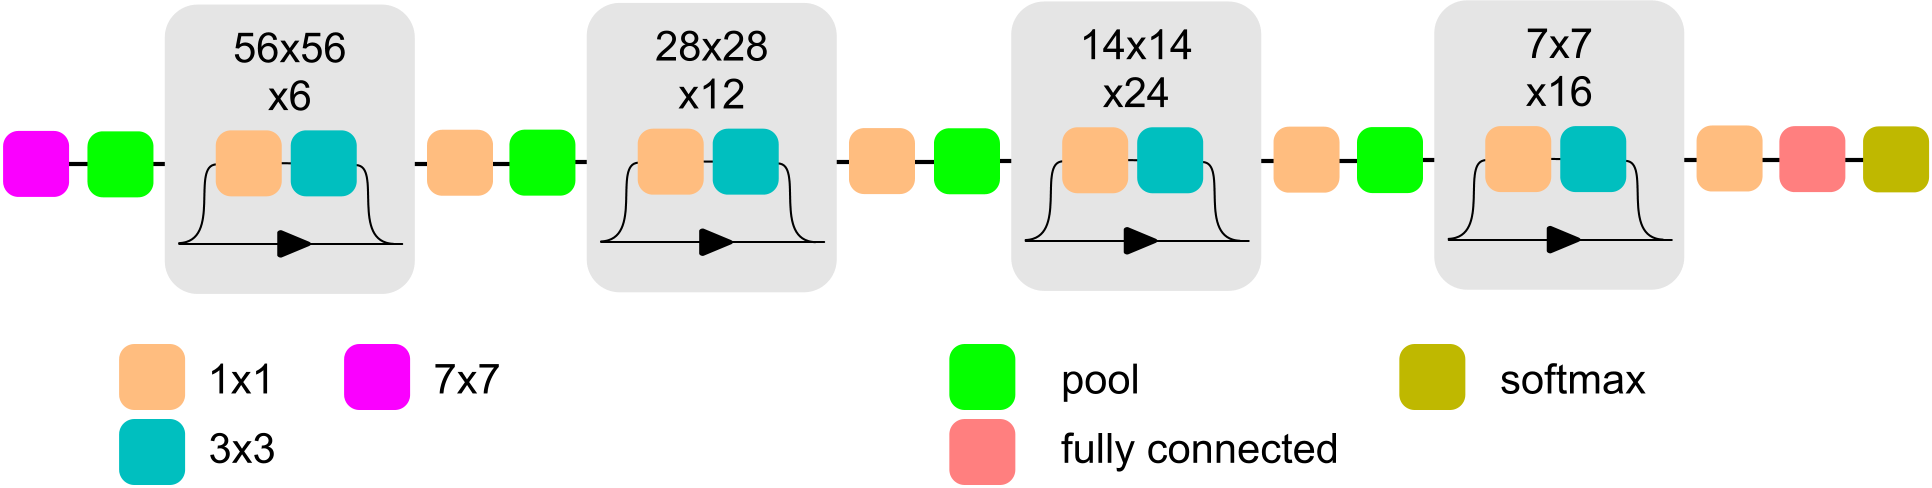
\includegraphics[width=0.8\linewidth]{densenet1}}
\caption{Архитектура сети DenseNet}
\label{img:densenet1}
\end{figure}

Быстрее обучается и точнее работает по сравнению с ResNet с аналогичным количеством параметров.
 
\end{frame}


\end{document}